\documentclass[../../../main]{subfiles}


\begin{document}
\subsection{Microcontroller Operating System}

The purpose of this section is to detail how the operating system for the Tiva microcontroller is setup and the reasoning behind those choices. The Tiva's responsibility is to act as the brain of the entire system while the FPGA acts like a data acquisitions device and a hardware controller.

The primary reasoning behind the choice of operating system is the need to run more than one task on the system. The system FreeRTOS is chosen partly due to the fact that this OS is part of another course and therefore beneficial to be familiar with, but also due to it allowing a preemption scheduler as opposed to a Run-To-Complete scheduler. At the time of the choice it was not clear whether the preemptive capability was going to be decisive and FreeRTOS provides both.
\\

FreeRTOS, an open source RealTime operating system created by Real Time Engineers LTD handles system, processes of different types by creating "Tasks" that are the run using a preemptive scheduler which allows the system to not only run multiple tasks in "parallel"\footnote{Due to only one core being supported by FreeRTOS, true parallel is not possible.} but also efficiently allocate the systems available resources.


A task is a single area of responsibility that either by necessity or by convention is combined as a single logical unit. Each task in the system, a full overview of these can be observed in the task diagram in figure \ref{fig:entire_task_diagram} can then be scheduled based on the priority it has been assigned and whether the task itself has decided that it wants to be scheduled.

\begin{figure}[H]
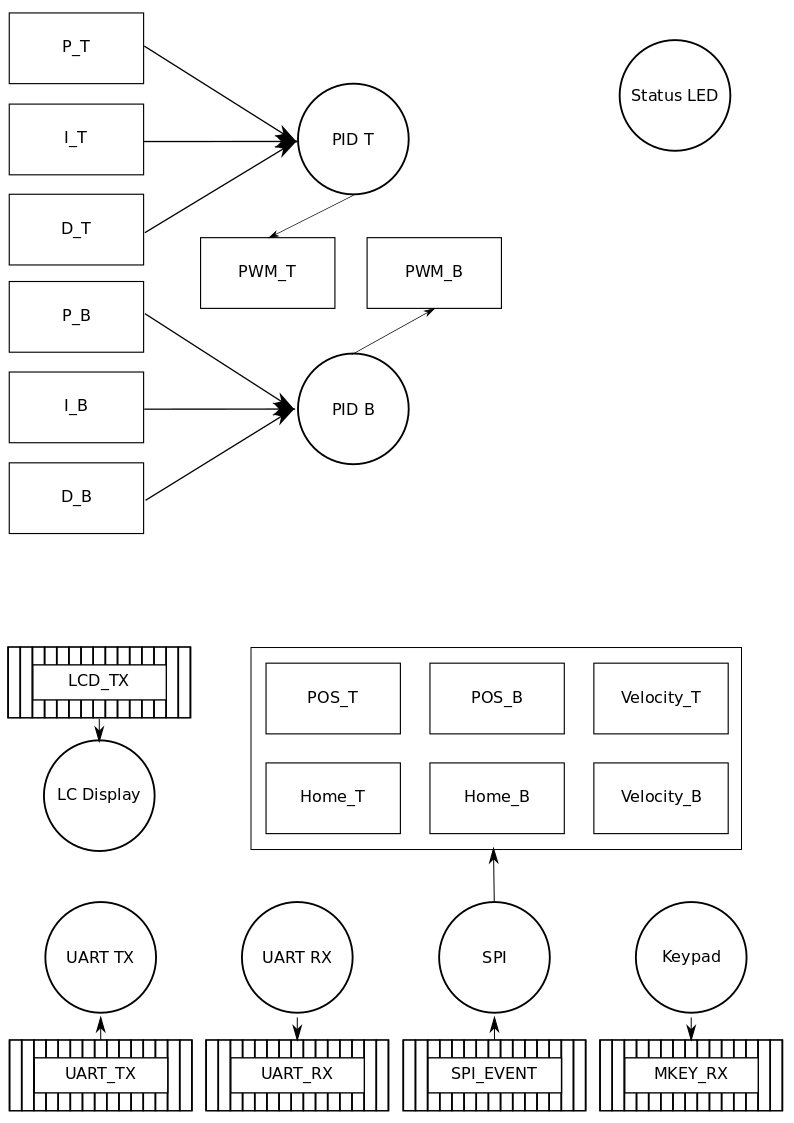
\includegraphics[width=0.9\columnwidth]{\main/afsnit/system_implementation/FreeRTOS/taskdiagram_full.png}
\caption{Task Diagram of entire system}
\label{fig:entire_task_diagram}
\end{figure}

\subsubsection{Scheduling}

In order to enable the microcontroller to run more then one task some form of scheduling must be implemented. This allows the operating system\footnote{FreeRTOS} to make a choice as to what tasks need processing capacity at this moment in time. In the FreeRTOS based system running on the Tiva scheduling is done through a priority based preemption capable implementation.

Preemption is when the operating system has the ability to pause execution of a process without the process willingly giving up CPU time. This allows time slicing without having the need for individual processes to be designed in a way to accommodate this. Further this allows the system to equally share time between long running processes.

The preemption capability enables the system to respond quickly to higher priority tasks becoming available for execution. This prevents waiting for the current task to return on its own potentially taking the CPU forever, the current task  will be paused and the higher priority task executed before the lower priority one is resumed and potentially completed.

As already mentioned the priority allows the system to select more important\footnote{Defined by the programmer} processes to be run quickly when such a task is available. 

The scheduler is run by a timer interrupt every 5ms and during this the current task is paused and the scheduler evaluates the next eligible task to run, this may be the same task that was running before and this will then be resumed, but the scheduler must be run every 5ms tick to ensure correct handling of priorities.

\subsubsection{Subtask Communication}

The multiple task architecture where each task deals only in their own specific area of the system requires since the combination of tasks are designed to accomplish one or more high level objective, a way to efficiently communicate between tasks running on the system.
This is accomplished using a combination of state buffers and queues.

State buffers are simple buffers keeping the last value written to it until a new value is overwrites this regardless of how many reads has been performed in that time. The implementation of this concept is done through variables of the appropriate task being declared in global scope and therefore available to every function in the system.

All queues in the system are FIFO\footnote{First-In-First-Out} queues which allows easy exchange of data between different parts of the system, while maintaining loose coupling between components. This loose coupling allows more parallel development and a more robust end product.

To maintain data integrity all shared-write resources are protected with semaphores allowing a task to obtain exclusive access to a resource and be able to update it without risk of data corruption caused by interrupted write access.
These semaphores are done via the implementation that ships with FreeRTOS and allows both binary and counting semaphores, although only the binary implementation is utilized.



\subsubsection{Tasks}

The entire system has been created as a task diagram in figure \ref{fig:entire_task_diagram}.

There is a number of task that exists only to provide services to other tasks, those tasks are designated system tasks.

Each task is designated a priority\footnote{by the designer} based on the demands of that particular task. The biggest consideration is the time sensitivity of the task, the need for timing to be consistent between runs. FreeRTOS in theory supports as many priority levels as RAM is available to handle. The recommendation from FreeRTOS is to not have more levels than needed. The system uses three levels in this implementation, LOW, NORMAL and HIGH. With HIGH providing the best timing accuracy due to the fact that it is a HIGH priority task  ready to run, then it will be run at the next scheduler run without having to wait for other tasks to potentially use up a time slice before its own run.


\paragraph{Status LED task}

This task only exist to toggle an LED on the board to verify that the OS is running and has not encountered some problem that could not be resolved automatically. Therefore the task has been assigned a low priority and will be processed with spare capacity.

\paragraph{UART Tasks}%

This group consists of the Transmit and Receive task, whom have been created completely independently. The TX task accepts data through a queue and sends that out the system by UART. The RX task is the inverse of this. These tasks are part of what makes the system work and therefore run with normal priority.

\paragraph{LCD Task}

The LCD task takes items from a queue and adds them to the currently active line on the LCD display. The task is run with low  priority as this only need to provide feedback in human observable time frames.

\paragraph{Matrix Keypad Task}

This task simply adds key presses from the keypad to a queue available to the rest of the system. It is being run with low priority as immediate response is not required for function.

\paragraph{Serial Peripheral Interface Task}

The SPI task handles all communication between the microcontroller and the FPGA and thus is indirectly responsible for all data acquisition and hardware control. This requires a priority of normal so the task is prioritized but does not require hard timing.\\

Besides system tasks there are tasks that can be categorized as being the "application" run on the system. These tasks are designated "user tasks".

\paragraph{PID}

This group of two tasks handle the control for both axis of the pan-tilt system and are the most critical processes. These run with high priority and therefore the best timing reliability that the system can offer.

\paragraph{User interface}


\end{document}
